% !TEX root = ../../../thesis.tex
    
%**************************************************************
% Methodology
%*************************************************************

\chapter{Valutazione}
    In questo capitolo vengono analizzate le metriche di valutazione prese in considerazione ai fini 
    dell'analisi del dataset reale delle richieste a servizi fatte a Infostud, la piattaforma su cui si fonda 
    la carriera accademica di tutti gli affiliati all'università La Sapienza.

    \section{Metriche di Valutazione}
        %**************************************************************
% Metriche di Valutazione
%**************************************************************

Nel contesto dell'analisi condotta sui dati osservati della piattaforma Infostud, è fondamentale valutare numericamente 
le soluzioni dei modelli applicati ai fini della valutazione delle loro performance. A tale scopo, vengono utilizzate 
tre metriche importanti: la precisione (precision), il richiamo (recall) e la F1-score (F1) al fine di misurare 
l'efficacia delle soluzioni in modo rigoroso. Queste metriche sono essenziali per comprendere in modo completo ed 
esaustivo l'efficacia degli approcci metodologici applicati.

\subsection{Precisione (Precision)}\label{precision}
    La precisione è una metrica che misura quanto un modello è accurato nel predire gli esempi positivi, o anomali nel 
    contesto dell'anomaly detection, rispetto a tutti 
    i casi che il modello ha classificato come positivi. 
    Per calcolare la precisione, viene valutata la frazione di predizioni positive fatte dal modello che sono effettivamente 
    corrette.
    \[Precision = \frac{TP}{TP+FP}\]\
    Dove:
    \begin{enumerate}
        \item TP (True Positives) rappresenta il numero di casi positivi, o anomali,
        correttamente classificati dal modello.
        \item FP (False Positives) sono i casi negativi erroneamente classificati come positivi, o anomali, dal modello.
    \end{enumerate}
    La precisione fornisce un riscontro numerico che, se massimizzato, rende il modello affidabile quando afferma 
    che un caso è positivo. Tuttavia, la precisione da sola potrebbe non fornire una visione completa delle prestazioni 
    di un modello.

\subsection{Richiamo (Recall)}
    Il richiamo misura la capacità di un modello di individuare tutti gli esempi positivi correttamente. In altre parole, 
    indica quanto il modello fornisce soluzioni che correttamente identificano gli esempi positivi. Il richiamo 
    viene calcolato attraverso la frazione di predizioni positive, o anomale, fatte 
    dal modello rispetto al totale dei casi positivi effettivi.
    \[Recall = \frac{TP}{TP+FN}\]
    Dove:
    \begin{enumerate}
        \item TP sono i True Positives, definiti nella \hyperref[precision]{Sottosezione 4.1.1}
        \item FN (False Negatives) rappresenta il numero di casi positivi, o anomali, erroneamente classificati come negativi 
              dal modello.
    \end{enumerate}
    Un alto valore di richiamo indica che il modello ha un'ottima capacità di individuare gli esempi positivi, ma 
    non tiene in considerazione il numero di casi falsi positivi.

\subsection{F1-Score (F1)}\label{f1-score}
    L'F1-score è una metrica che combina la precisione e il richiamo in un valore che tiene conto sia dei falsi positivi 
    che dei falsi negativi. La metrica bilancia la precisione e il richiamo. La formula per calcolare l'F1-score è 
    la seguente:
    \[F1 = \frac{2\cdot Precision \cdot Recall}{Precision+Recall}\]
    L'F1-score, quindi, mira a cercare un compromesso tra i valori di precisione e richiamo.



    \section{Valutazione del modello statistico ARMA}
        %**************************************************************
% Valutazione ARMA
%**************************************************************

Come è stato già osservato, il modello statistico ARMA racchiude in modo discreto il comportamento del dataset e indica come anomalie i casi in 
cui la previsione del modello si discosta molto dai dati reali. In particolare, gli iperparametri scelti 
hanno riportato uno score F1 di 0.750 sul dataset di validation, mentre 
le metriche osservate sull'insieme di test sono riportate nella \hyperref[tab:arma-metrics]{Tabella 4.1.}

\begin{table}[H]
    \centering
    \caption{Risultati ARMA.}
    \begin{tabular}{lr}
    \toprule
    \textbf{Soluzione ARMA sul test set}  \\
    \midrule
    \multirow{3}{*}{\textbf{Metriche}} & Precisione: 0.332 \\
    & Recall: 0.248 \\
    & F1-score: 0.284 \\
    \bottomrule
    \end{tabular}
    \label{tab:arma-metrics}
\end{table}

I risultati mostrano che ARMA riesce a catturare la tendenza generale del modello e molti 
andamenti anomali vengono predetti come tali. La soluzione non è ottimale, ma fornisce 
comunque una buona base per la valutazione di MSCRED.

    \section{Valutazione del modello ML OC-SVM}
        %**************************************************************
% Valutazione OC-SVM
%**************************************************************

Il metodo che si basa sul machine learning, One-Class Support Vector Machine, arricchisce l'analisi e lo studio 
delle anomalie sul daset di Infostud fornendo una soluzione molto buona sull'insieme di validazione con uno score F1 pari 
a 0.716, e una discreta sull'insieme di test, come mostrato nella 
\hyperref[tab:ocsvm-metrics]{Figura 4.2.}


\begin{table}[H]
    \centering
    \caption{Soluzione OC-SVM.}
    \begin{tabular}{lr}
    \toprule
    \textbf{Soluzione OC-SVM sul test set}  \\
    \midrule
    \multirow{3}{*}{\textbf{Metriche}} 
        & Precisione: 0.331 \\
        & Recall: 0.290 \\
        & F1-score: 0.309 \\
    \bottomrule
    \end{tabular}
    \label{tab:ocsvm-metrics}
\end{table}

I risultati mostrano che OC-SVM è in grado di produrre buoni risultati durante la fase di 
validazione ma fallisce durante la fase di test. Tuttavia, è importante notare che il modello è stato applicato 
in un contesto avverso, caratterizzato da un forte sbilanciamento tra le classi. Nonostante l'ambiente sfavorevole, 
questa soluzione è un punto di riferimento ragionevole per valutare le prestazioni del modello MSCRED.

    \section{Valutazione del modello DL Telemanom}
        %**************************************************************
% Valutazione Telemanom
%**************************************************************

Gli iperparametri ottimali applicati al dataset interessato hanno generato una buona soluzione come evidenziato nella
    \hyperref[tab:telemanom-metrics]{Tabella 4.3.}

    \begin{table}[H]
        \centering
        \caption{Risultati Telemanom.}
        \begin{tabular}{lr}
        \toprule
        \textbf{Soluzione Telemanom sul test set}  \\
        \midrule
        \multirow{3}{*}{\textbf{Metriche}} 
            & Precisione: 1.0 \\
            & Recall: 0.5 \\
            & F1-score: 0.66 \\
        \bottomrule
        \end{tabular}
        \label{tab:telemanom-metrics}
    \end{table}

La soluzione sembra ottima, notevolmente migliore rispetto a quelle dei modelli precedenti, tuttavia non è totalmente 
valida nella nostra applicazione e il motivo è semplice: Telemanom gestisce le anomalie, e calcola metriche su esse,
basandosi solo sugli intervalli anomali come già citato nella \hyperref[sez-telemanom]{Sottosezione 3.3.1}. Gli intervalli anomali ground-truth
nell'esperimento appena riportato sono solo due: uno grande che dura considerevolmente nel tempo, mentre l'altro 
molto più piccolo, come si evince nella \hyperref[fig:telemanom-ys-comparison]{Figura 4.1.}, in cui 
sono illustrati i valori reali e i valori previsti dal modello del dataset che rappresenta la latenza media 
delle richieste di login a Infostud. Telemanom identifica sempre e solo l'intervallo più grande come anomalo 
nei modelli dei vari canali, mentre quello più piccolo non è mai rilevato. Ciò ha portato a una soluzione che
sembra ottima, ma che in realtà, per struttura stessa del modello e dei dati che osserva, sta overfittando il 
dataset. Nella \hyperref[fig:telemanom-e_s]{Figura 4.2.} viene illustrato il grafico degli errori
smussati $\mathbf{e}_s$ riferente allo stesso segnale precedente.

\begin{figure}[H]
    \centering
    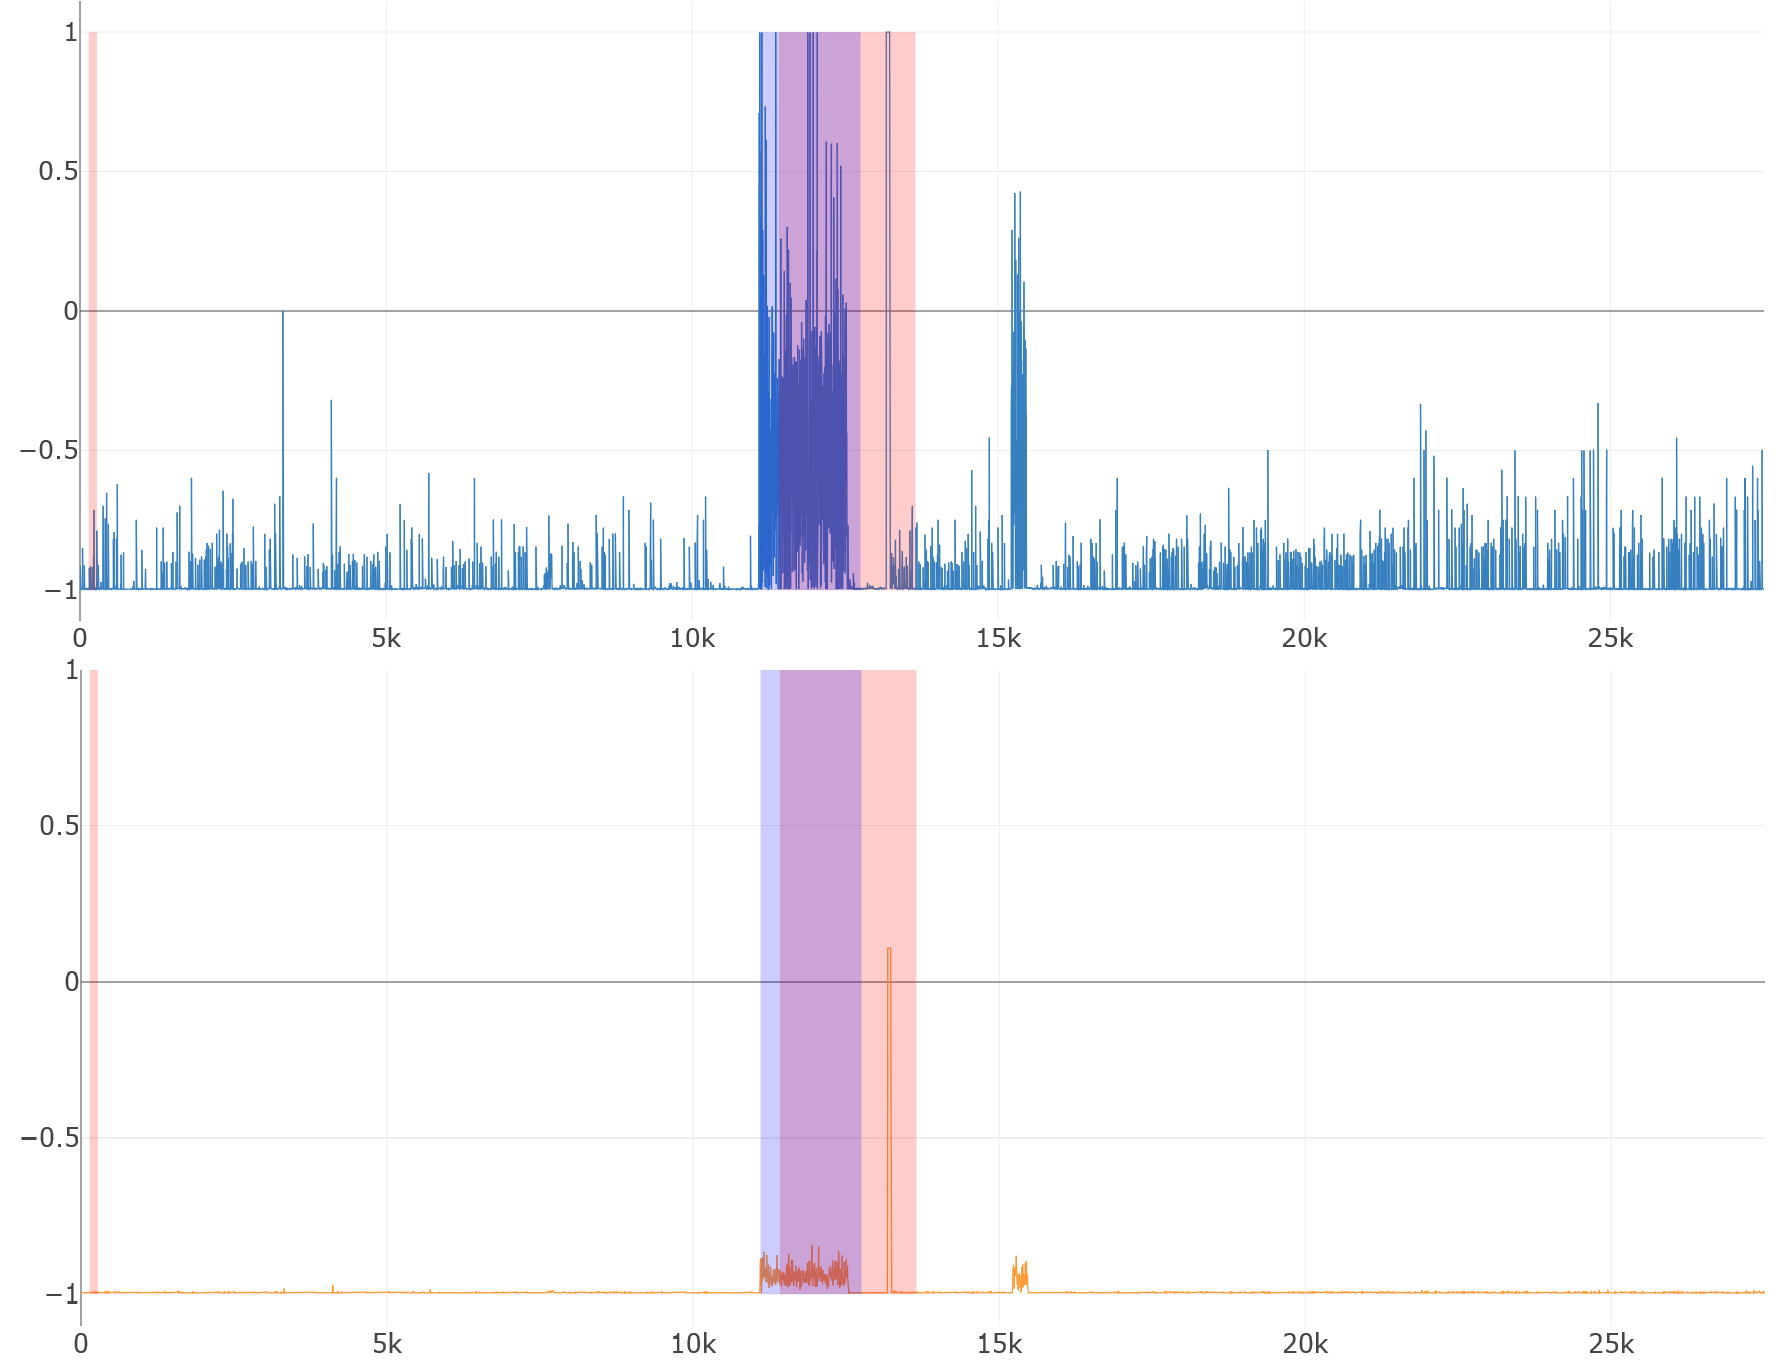
\includegraphics[width=0.7\textwidth]{./input/chapters/models/figs/telemanom-ys-comparison.png}
    \caption{Dati reali $y$ (sopra) e previsione di Telemanom $\hat{y}$ (sotto) della latenza media delle richieste
    login a InfoSapienza. Le bande rosse rappresentano periodi anomali ground-truth, la banda blu è l'intervallo 
    che il modello giudica anomalo.}
    \label{fig:telemanom-ys-comparison}
\end{figure}

\begin{figure}[H]
    \centering
    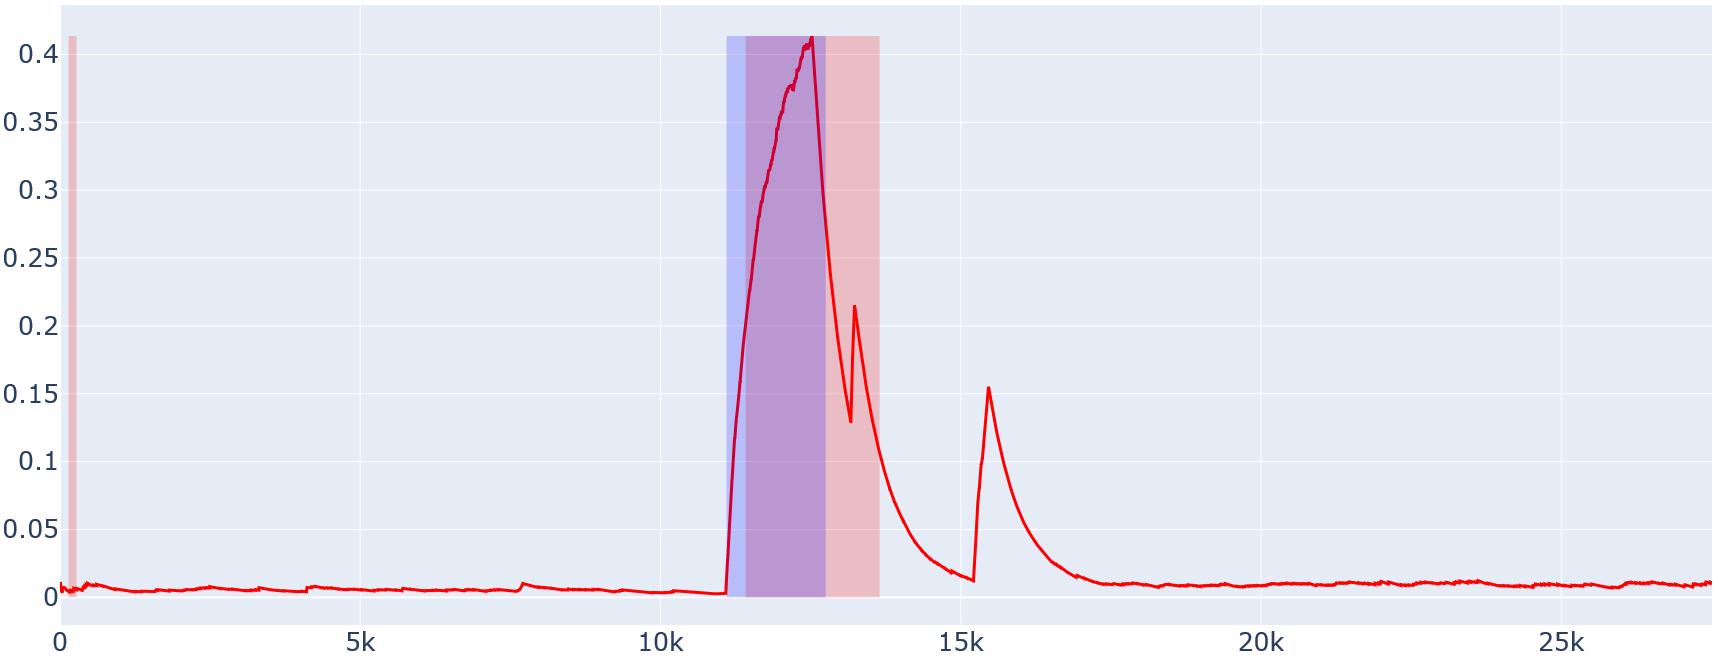
\includegraphics[width=0.7\textwidth]{./input/chapters/models/figs/telemanom-e_s.png}
    \caption{Errore smussato tra i valori reali e la previsione del modello $\mathbf{e}_s$ dei dati che rappresentano la 
    latenza media delle richieste login a InfoSapienza.}
    \label{fig:telemanom-e_s}
\end{figure}


Durante il mio studio di Telemanom ho compreso che il modello, in un contesto in cui sono presenti più anomalie 
che non durano molto nel tempo non performa in maniera altrettanto ottimale. Per riuscire a ottenere un 
discreto punteggio di recall, viene generato un grande numero di falsi positivi; i risultati rimangono coerenti 
a ciò che gli autori originali hanno descritto nel paper: Telemanom, purtroppo, genera molti falsi positivi, e non sembra che 
le sue capacità di pruning, nell'ambito di InfoSapienza, riescano a mitigare molto il problema.
    
In sintesi Telemanom, purtroppo, non si presta bene nel contesto della rilevazione di anomalie 
del dataset di Infostud. Il risultato, seppur ottimo, non viene ritenuto valido perché genera una soluzione che, 
in una situazione più naturale, sarebbe stata molto diversa.
    \section{Valutazione del modello DL MSCRED}
        %**************************************************************
% Valutazione MSCRED
%**************************************************************
\label{val-mscred}
Dopo 7 epoche di addestramento, MSCRED ha proposto la soluzione riportata in \hyperref[fig:sol-valid-mscred]{Figura 4.3.} per l'insieme 
di validazione. Evidenziamo come MSCRED riesca a percepire l'andamento improvvisamente anomalo della serie temporale estratta 
dal dataset di Infostud, 
generando anomaly score elevati per ogni punto corrispondente a uno dei ventisei delle anomalie ground-truth, 
evidenziate dall'area rossa. In questo caso, la soluzione ha portato a un risultato perfetto, ottenendo uno score 
F1 pari a 1.0 e affermando l'ipotesi sollevata nel \hyperref[cap2:hypothesis]{Capitolo 2}: il dataset che rappresenta 
le latenze medie è un ottimo indicatore per quanto riguarda l'analisi e l'individuazione delle anomalie.

Riguardo all'insieme di test, MSCRED ha ottenuto risultati leggermente inferiori ma propone comunque una soluzione ottima 
mostrata in \hyperref[fig:sol-test-mscred]{Figura 4.4.} Le metriche risultanti dalla soluzione sono riportate 
nella \hyperref[tab:mscred-metrics]{Tabella 4.4.}

\begin{figure}[H]
    \centering
    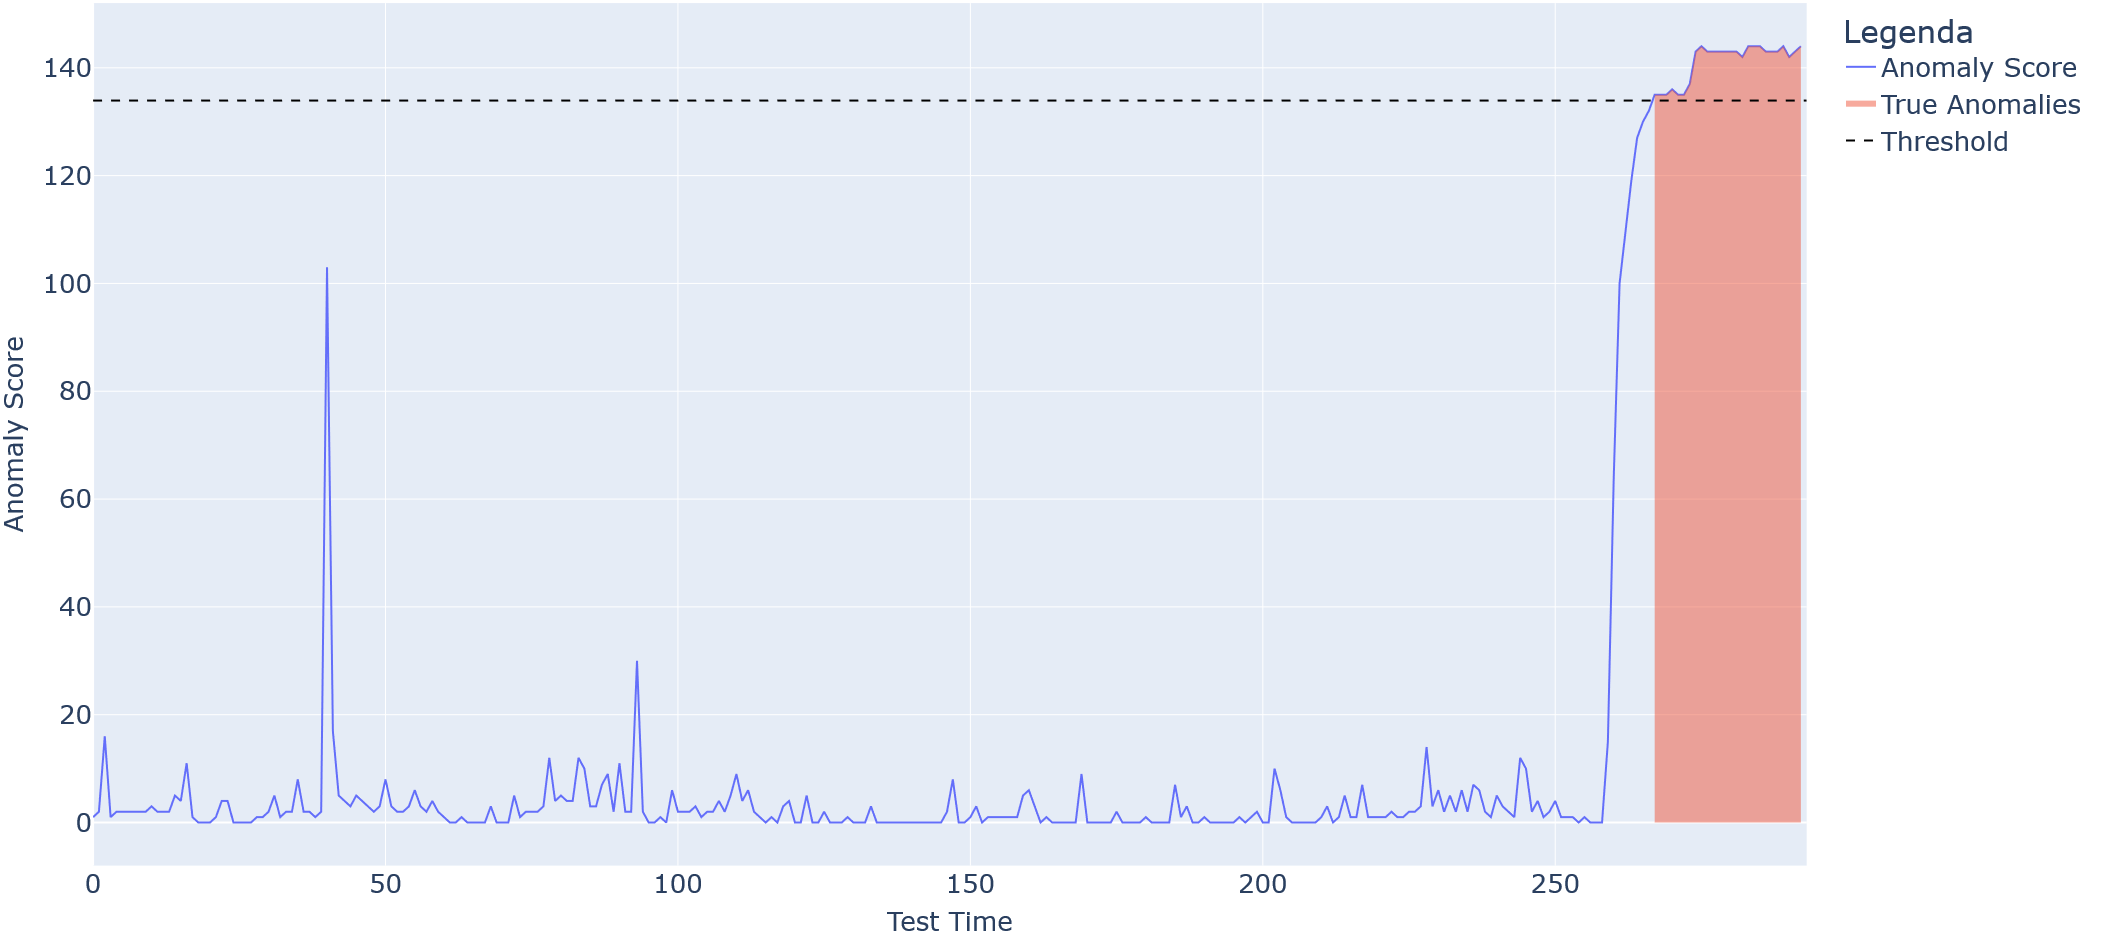
\includegraphics[width=0.7\textwidth]{./input/chapters/models/figs/sol-valid-mscred.png}
    \caption{Soluzione MSCRED sul validation set.}
    \label{fig:sol-valid-mscred}
\end{figure}


\begin{figure}[H]
    \centering
    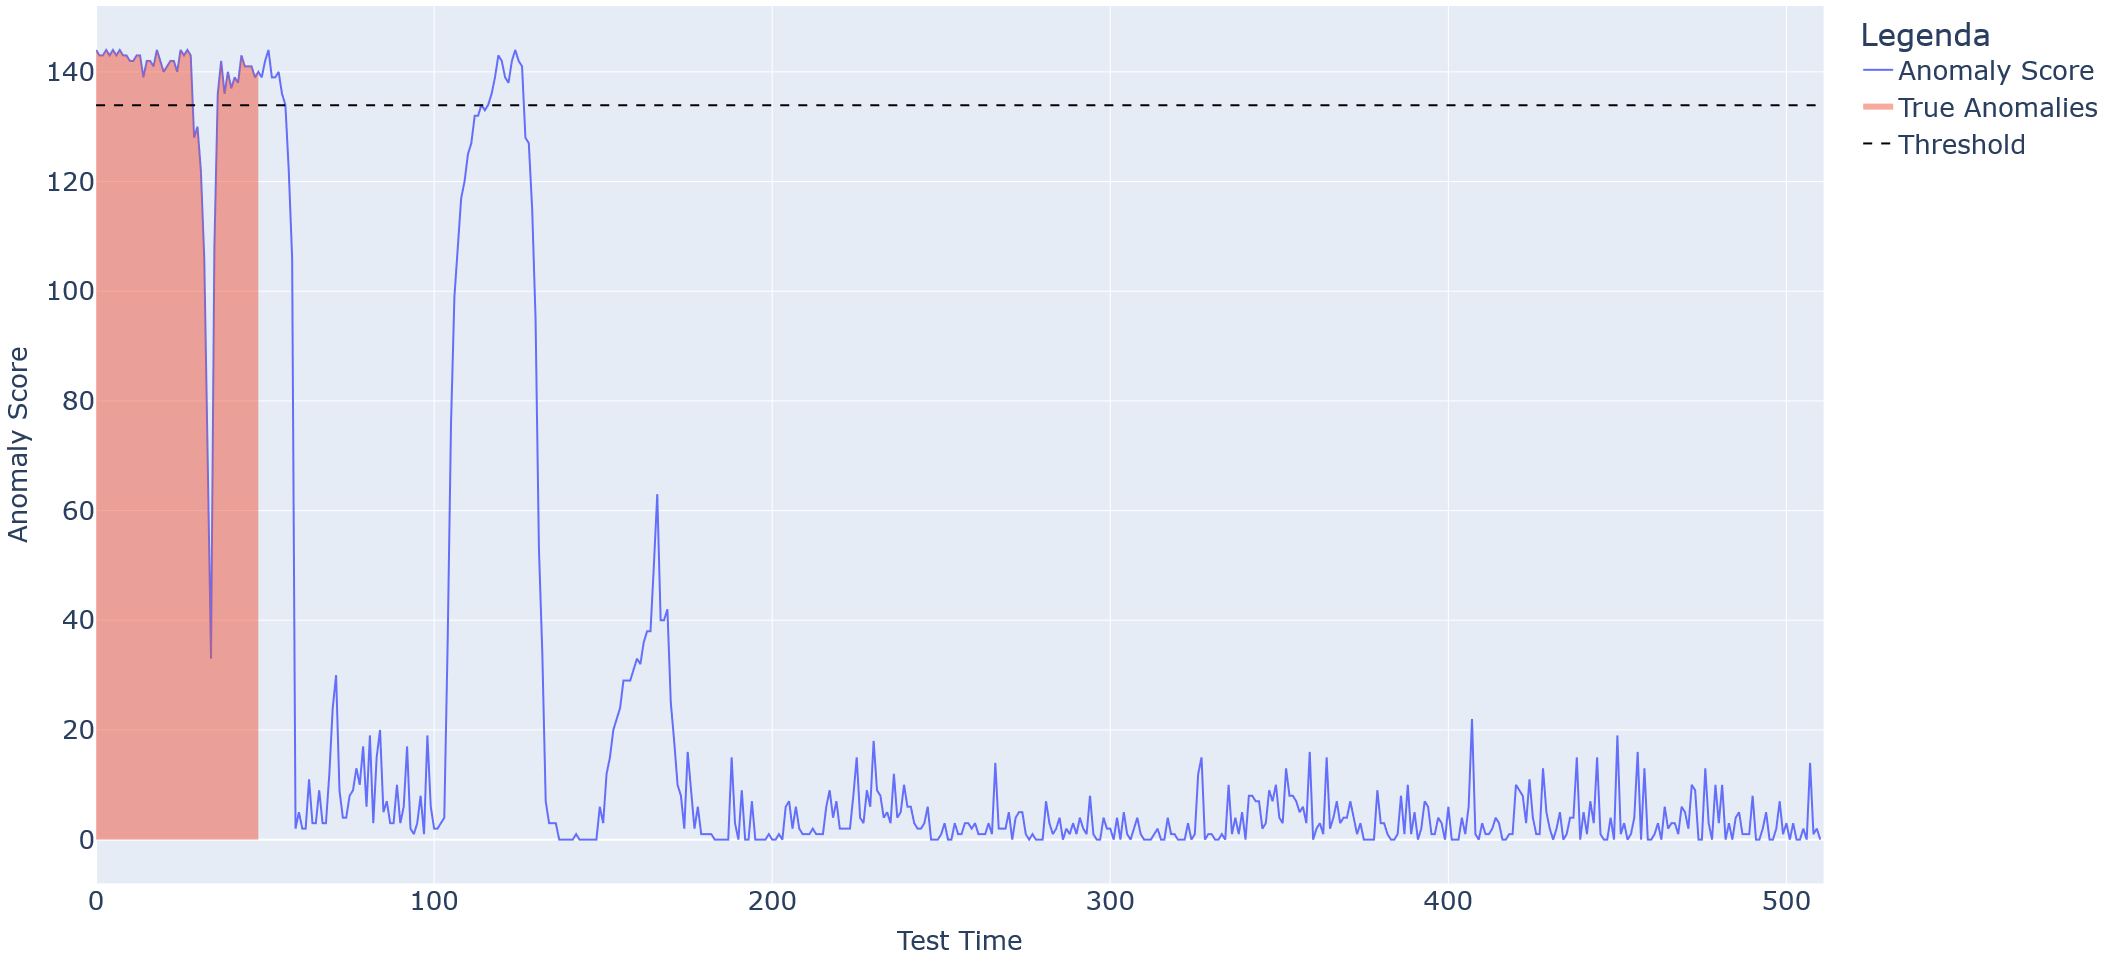
\includegraphics[width=0.7\textwidth]{./input/chapters/models/figs/sol-test-mscred.png}
    \caption{Soluzione MSCRED sul test set.}
    \label{fig:sol-test-mscred}
\end{figure}

\begin{table}[H]
    \centering
    \caption{Risultati MSCRED.}
    \begin{tabular}{lr}
    \toprule
    \textbf{Soluzione MSCRED sul test set}  \\
    \midrule
    \multirow{3}{*}{\textbf{Metriche}} & Precisione: 0.711 \\
    & Recall: 0.857 \\
    & F1-score: 0.777 \\
    \bottomrule
    \end{tabular}
    \label{tab:mscred-metrics}
\end{table}

\paragraph{Conclusioni} I risultati dimostrano in maniera cristallina che MSCRED fornisce
soluzioni notevolmente migliori rispetto agli altri metodi presi in analisi.
Il modello, inoltre, riesce a catturare l'intercorrelazione dei segnali e la dipendenza temporale che
hanno le osservazioni vicine nello spazio, e quindi nel tempo, delle serie temporali multivariate.
MSCRED offre una misura numerica della severità delle anomalie anziché una semplice classificazione binaria, 
soddisfacendo così tutti i requisiti per un algoritmo di rilevamento delle anomalie discussi nel 
\hyperref[cap:intro]{Capitolo 1.} e permettendo all'anomaly detection di compiere un grande passo avanti. 

D'altro canto, però, assumendo che il dataset di Infostud preso in analisi rispetti 
la proprietà IID, MSCRED sembra non offrire soluzioni altrettanto ottimali su serie temporali molto lunghe, ma fa sì che alcune anomalie pesino 
molto più di altre e non garantisce più una netta differenza tra i periodi anomali e non anomali. Questa supposizione 
è basata su delle prove fatte durante il percorso di studio di MSCRED: più è lunga la serie temporale, più 
MSCRED sembra performare in maniera peggiore. Tale affermazione, però, richiede studi più approfonditi per poter 
essere dimostrata o smentita.